\documentclass[a4paper,12pt,oneside]{report}
\usepackage[magyar]{babel}
\usepackage[utf8]{inputenc}
\usepackage{t1enc}
\def\magyarOptions{defaults=hu-min}
\usepackage{cite}
\usepackage{amsmath,amssymb,amsfonts}
\usepackage{algorithmic}
\usepackage{graphicx}
\usepackage{textcomp}
\usepackage[dvipsnames]{xcolor}
%\usepackage{booktabs}
\usepackage{tabularray}
\usepackage{listings}
\lstset
{
	framexleftmargin=10mm,
	frame=shadowbox,
	rulesepcolor=\color{olive8},
	language=C,
	numbers=left,
	stepnumber=1,
	showstringspaces=false,
	tabsize=4,
	breaklines=true,
	breakatwhitespace=false,
	basicstyle=\footnotesize\ttfamily
}
\frenchspacing
\linespread{1.25}
\UseTblrLibrary{booktabs}
\usepackage[left=2.5cm,top=4cm,right=2.5cm,bottom=4.5cm,headsep=2cm]{geometry}

\usepackage{titlesec, blindtext, color}
\definecolor{gray75}{gray}{0.75}

\usepackage{fancyhdr}

\usepackage{etoolbox}
\patchcmd{\chapter}{\thispagestyle{plain}}{\thispagestyle{fancy}}{}{}

\begin{document}

\pagestyle{fancy}
\fancyhead[]{}
\fancyhead[C]{\thepage}
\fancyfoot[]{}
\fancyfoot[]{}
\renewcommand{\headrulewidth}{0pt}
\renewcommand{\footrulewidth}{0pt}

\titleformat{\chapter}[hang]{\normalsize\bfseries}{\color{Black}\thechapter .\hspace{10pt}}{0pt}{\normalsize\bfseries\color{Black}\MakeUppercase}

\titleformat{\section}[hang]{\normalsize\bfseries}{\hspace{0pt} \thesection .\hspace{10pt}}{0pt}{\normalsize\bfseries\MakeUppercase}

\titleformat{\subsection}[hang]{\normalsize\bfseries}{\hspace{0pt} \thesubsection .\hspace{10pt}}{0pt}{\normalsize\bfseries}

\title{Szakdolgozat}

\author{Tórizs Dániel György}

\date{}

\maketitle

\tableofcontents

\chapter{Bevezetés}

Az ezt megelőző félévekben elkezdett okosotthon projekt folytatása az idei évi is, amely jelenleg egy Raspberry PI-t tartalmaz.
Idén ennek a megismerésével foglalkoztam, valamint a node-REDdel. Ezek bemutatását tartalmazza majd ez a dokumentáció.

%\begin{itemize}

%	\item{Első bullet point}

%	\item{Második bullet point}

%	\item{Végül a harmadik}

%\end{itemize}

%És kódot is. Ilyenkor a LaTeX szépen sorszámozza nekünk, és egy keretet is tesz.
%(A sorszámozás, a keret, a behúzás stb. beállítható.)

%Ez egy kis térköz
%\medskip

%Így tudunk kódot beszúrni
%\begin{lstlisting}
%#include <stdio.h>
%int main()
%{
%	// printf() displays the string inside quotation
%	printf("Hello, World!");
%	return 0;
%}
%\end{lstlisting}

\chapter{Telepítés}

Az alaphoz egy Raspberry PI-t használtam, ezt az eszközt az Egyesült Királyságban fejlesztették ki oktatási célokra, igazából
egy bankkártya méretű számítógép amely különböző Linux operációs rendszerekkel képes üzemelni.

A telepítéshez a Raspberry PI Imagert használtam, ami egy elég egyszerű program.

\begin{figure}[htbp]
	\centering
	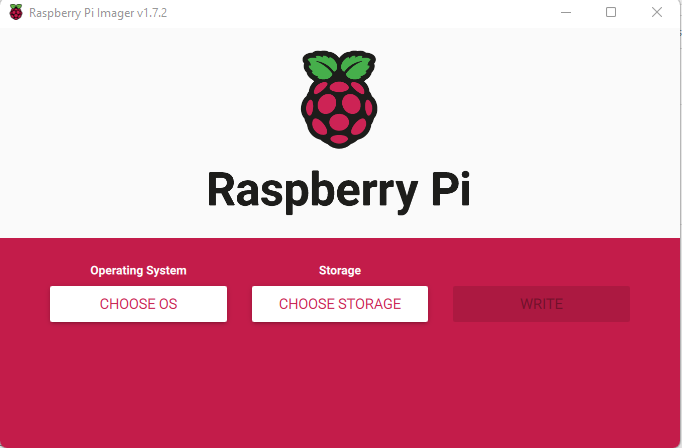
\includegraphics[width=0.35\textwidth]{fig/Imager.png}
	\caption{A telepítő program.}
	\label{fig-Imager}
\end{figure}

A programon bellül ki kell választanunk az operációs rendszert amit a Raspberry-n futtatni szeretnénk, ezen kívül a memóriakártyát, 
ami a háttértárunk lesz. Amikor ezzel megvagyunk még a beállításokban meg kell adnunk az eszköznek egy felhasználónevet és egy jelszót
valamint a router hozzáférési adatait.

\begin{figure}[htbp]
	\centering
	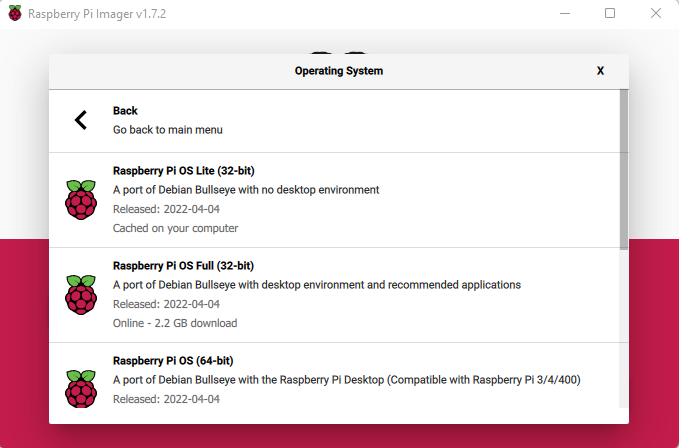
\includegraphics[width=0.35\textwidth]{fig/os.png}
	\caption{Operációs rendszerek.}
	\label{fig-os}
\end{figure}

Ha ezzel megvagyunk akkor elindul egy lassabb telepítési folyamat, amely a memóriakártyára helyezi az operációs rendszert, ezután pedig
egy ellenörzési folyamat, hogy minden rendben van-e.
Miután ezzel megvagyunk a memóriakártyát behelyezzük a Raspberry-be, ahol egy lassabb boot után elindul az eszköz (amikor ez megtörtént
akkor a led egy biztos ritmusra villog), ezután megkezdhetjük a hozzáférést az eszközhöz. 
A hozzáféréshez szükségünk van a router kezelőfelületére, ahol meg kell keresnünk az eszközünket, a legjobb ha adunk neki
egy saját nevet. Miután ez megvan a PuTTY segítségével hozzáférünk a Raspberry operációs rendszeréhez.

\begin{figure}[htbp]
	\centering
	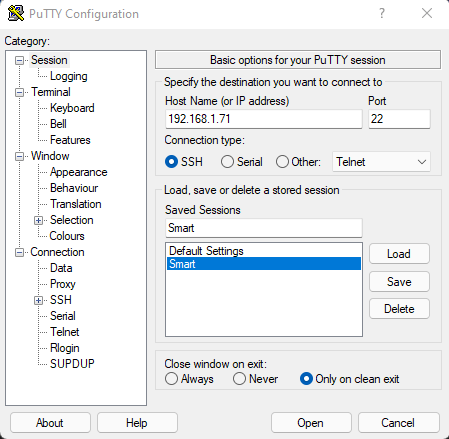
\includegraphics[width=0.35\textwidth]{fig/putty.png}
	\caption{PuTTY beállítás.}
	\label{fig-putty}
\end{figure}

\chapter{node-RED}

A node-RED egy áramlás alapű fejlesztő környezet ahol grafikusan tudunk programot készíteni egy böngésző segítségével. Eredetileg az IBM
készítette. Az elkészítet programokat egy JSON fájlban tárolja.

Az első node-RED-es próbálkozás egy egyszerű Hello, World! volt amihez igazából egy input és egy output részre van szükség.
Az input részben megadjuk a stringet ami az üzenetünk és a két részt összekötjük. A Deploy gombra kattintva tudjuk elindítani a
programunkat, ezután pedig az input előtti gombbal be is kapcsoljuk, ekkor megjelenik a Hello, World! felirat.

\begin{figure}[htbp]
	\centering
	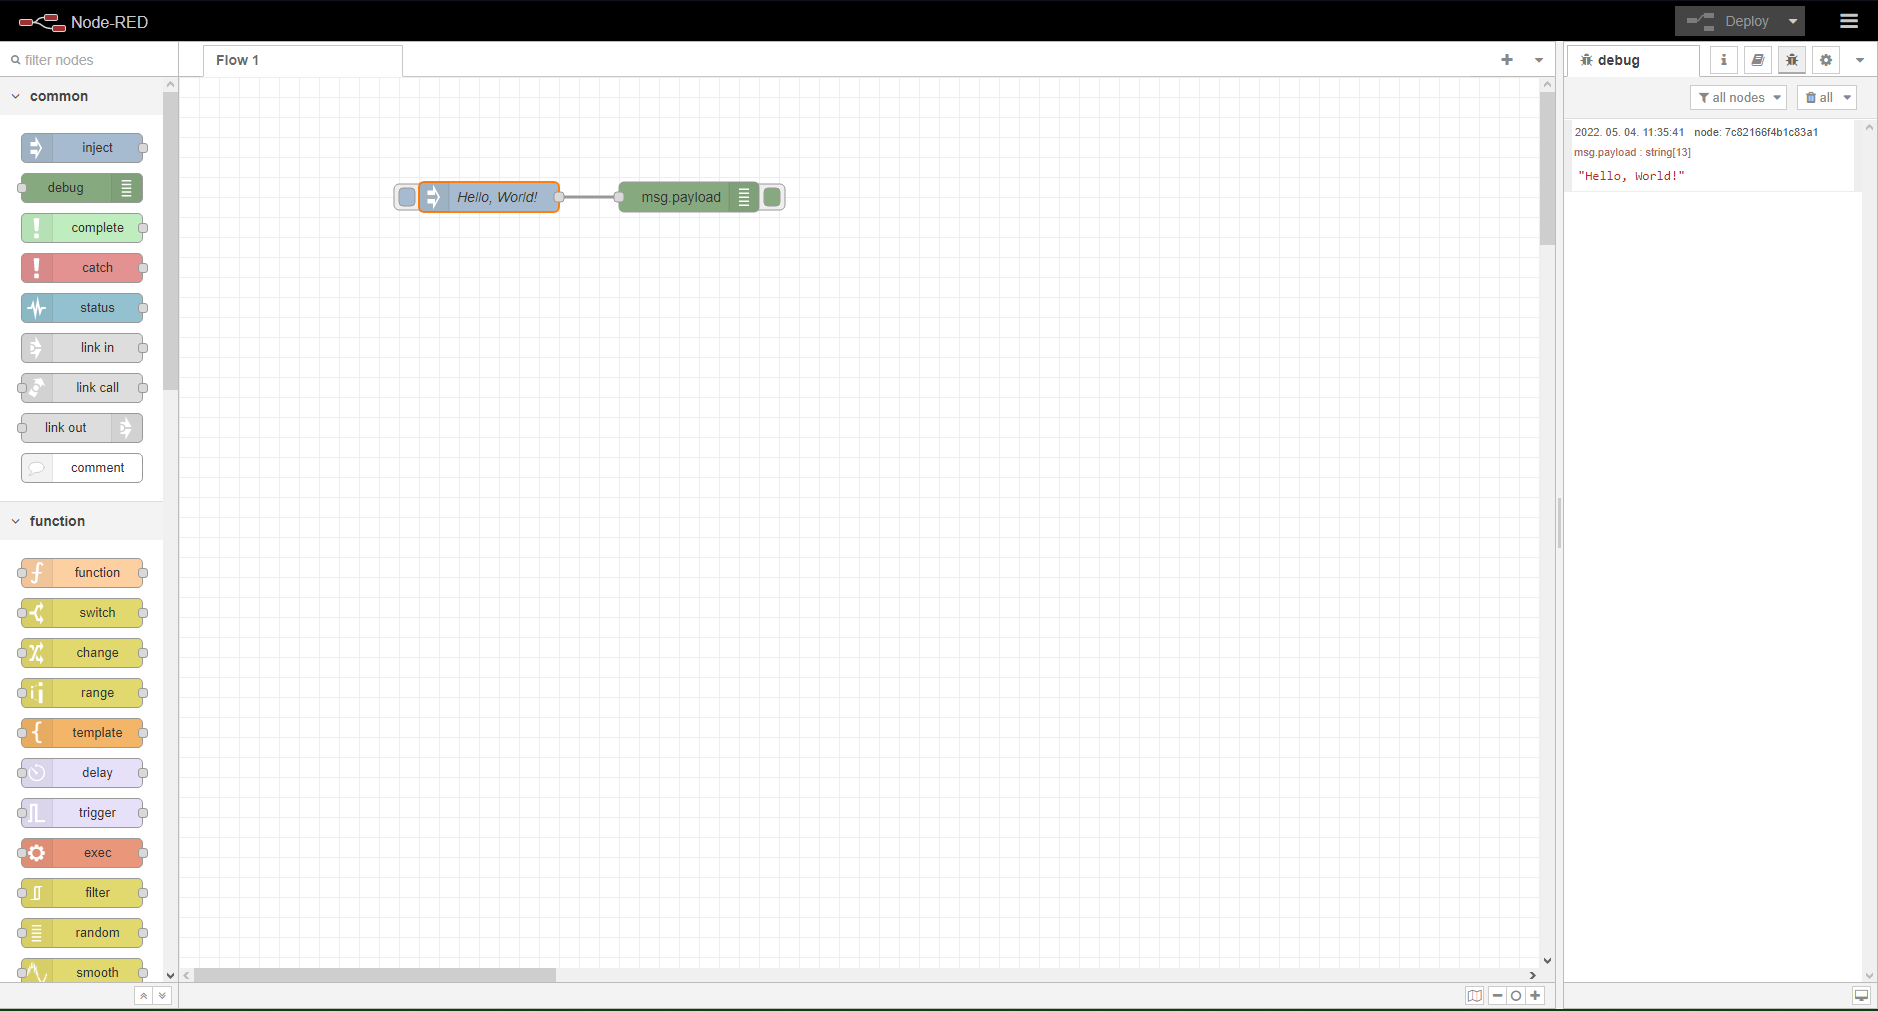
\includegraphics[width=0.35\textwidth]{fig/Hello, World.png}
	\caption{Hello, World!}
	\label{fig-Hello, World}
\end{figure}

A második részben több inputot használtam, hogy számokat tudjak bevinni egy outputra. A módszer haszonló mint az előzőnél
csak itt számokat használtam. Működés szempontjából mindig egy számot kaptunk a kimeneten, mindig azt a számot, amely input előtti
gombot megnyomtuk.

\begin{figure}[htbp]
	\centering
	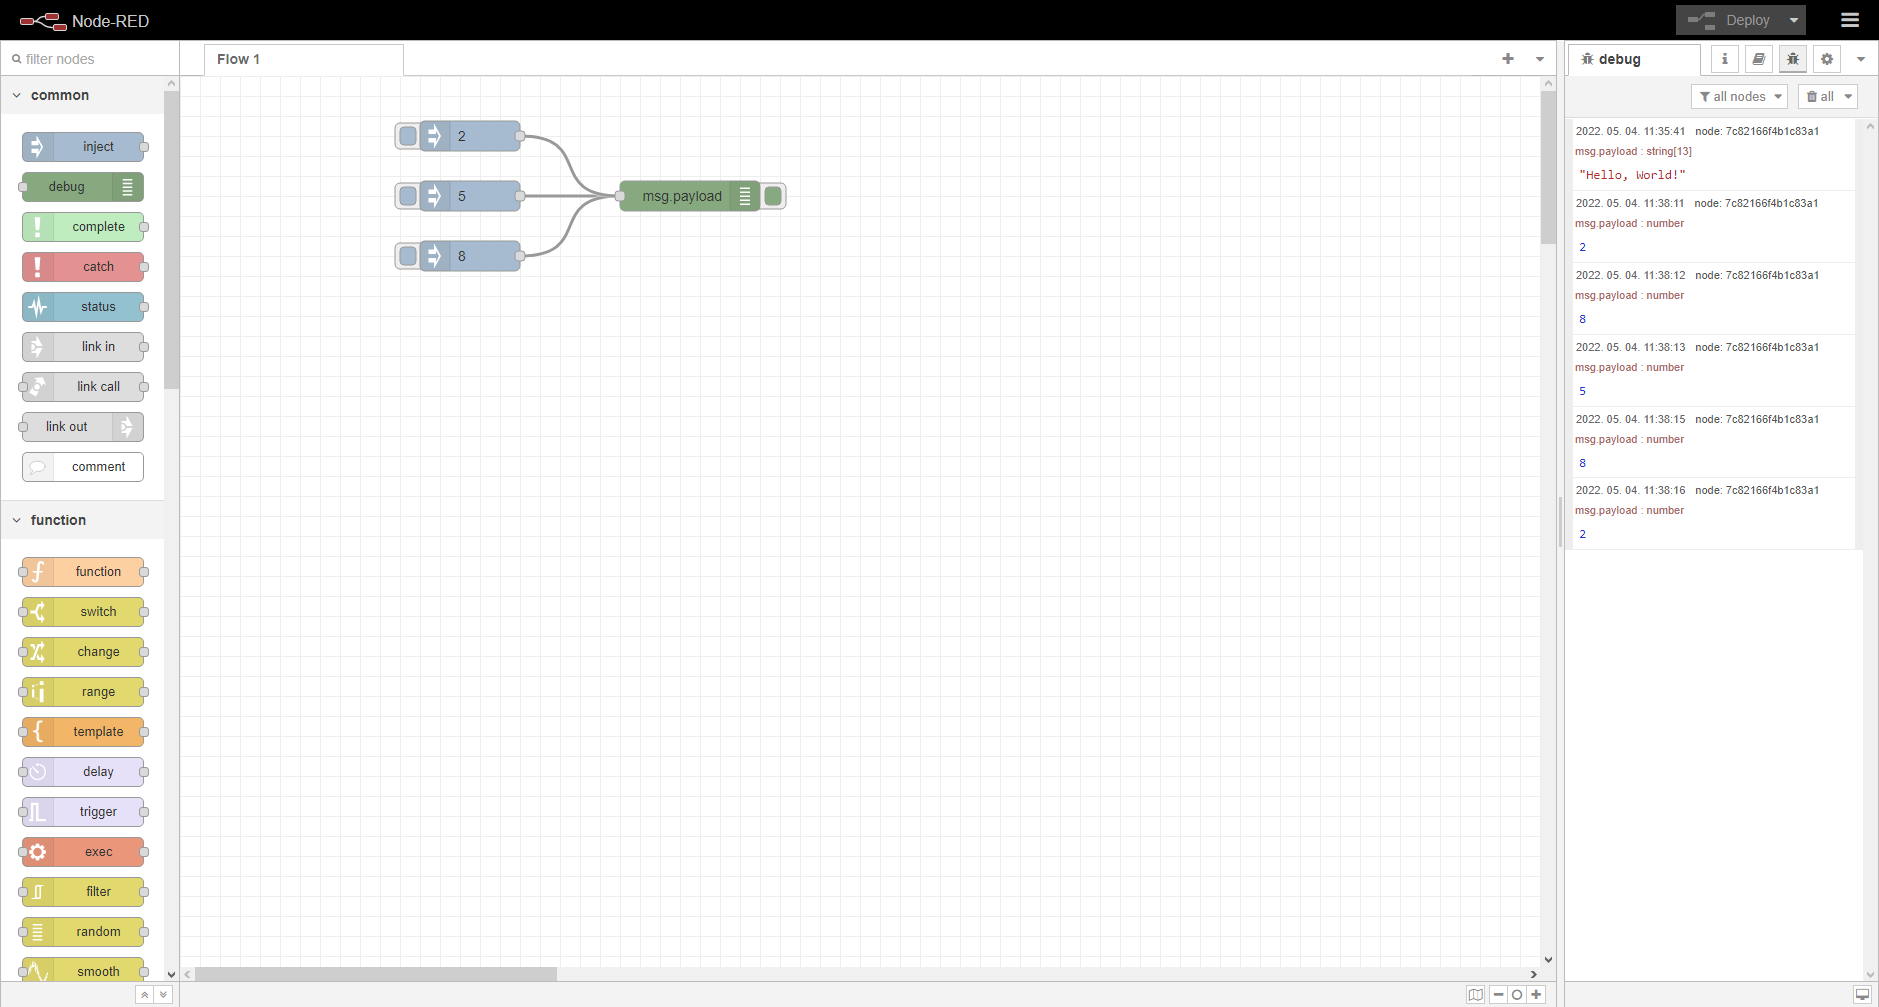
\includegraphics[width=0.35\textwidth]{fig/Numbers.png}
	\caption{Számok bevitele.}
	\label{fig-Numbers}
\end{figure}

A harmadik rész már egy komplexebb program, itt egy UI is van, valamint egy Chart. Az előző programból ismert számos módszer
itt is szerepel viszon ez nem csak kimenetre, hanem egy chartra is rá van kötve. Ha a bemeneten lévő gombok valamelyikét megnyomjuk 
akkor az adott szám megjelenik a grafikonon, ha pedig egyszerre többet megnyomunk akkor egy vonaldiagrammot rajzol nekünk.

\begin{figure}[htbp]
	\centering
	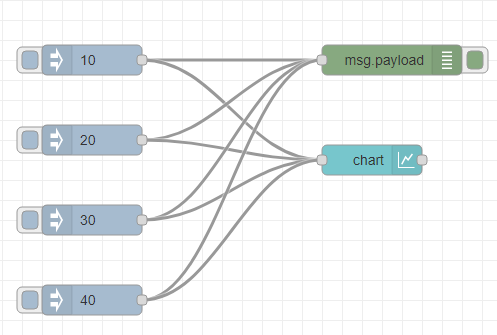
\includegraphics[width=0.35\textwidth]{fig/uichart.png}
	\caption{UI program.}
	\label{fig-uichart}
\end{figure}

\begin{figure}[htbp]
	\centering
	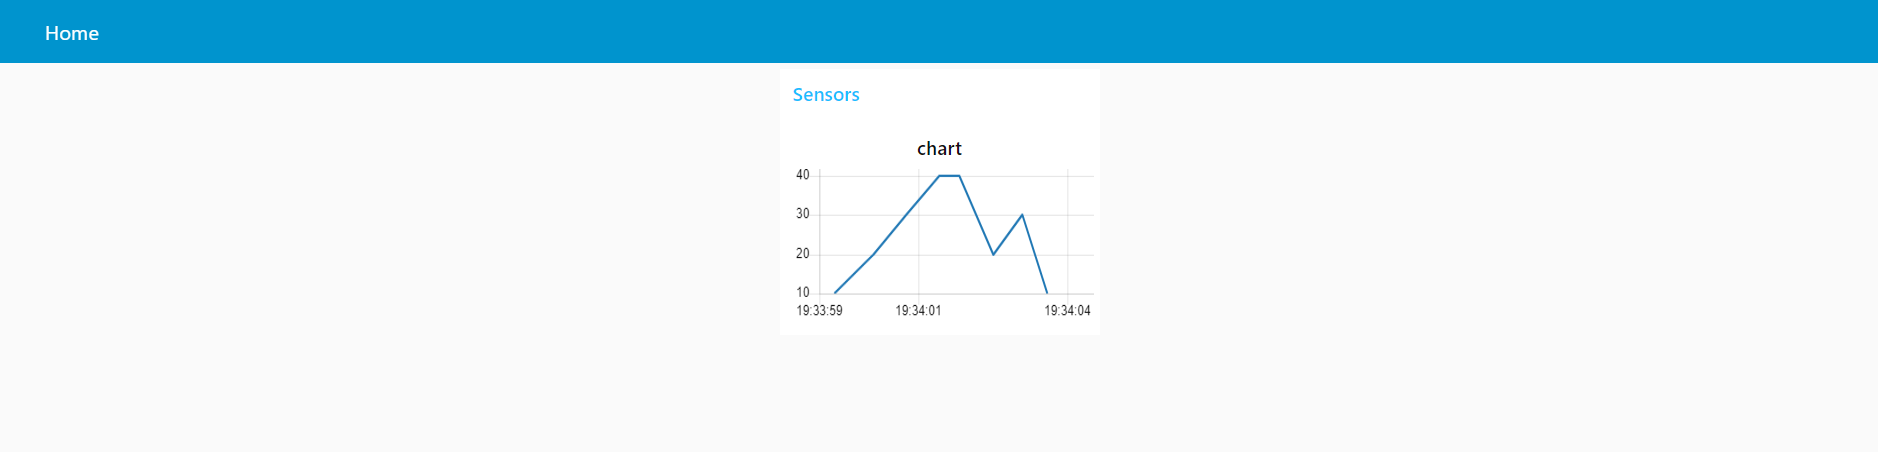
\includegraphics[width=0.35\textwidth]{fig/chart.png}
	\caption{A gombok véletlenszerű megnyomása utáni adatok.}
	\label{fig-chart}
\end{figure}



\begin{figure}[htbp]
	\centering
	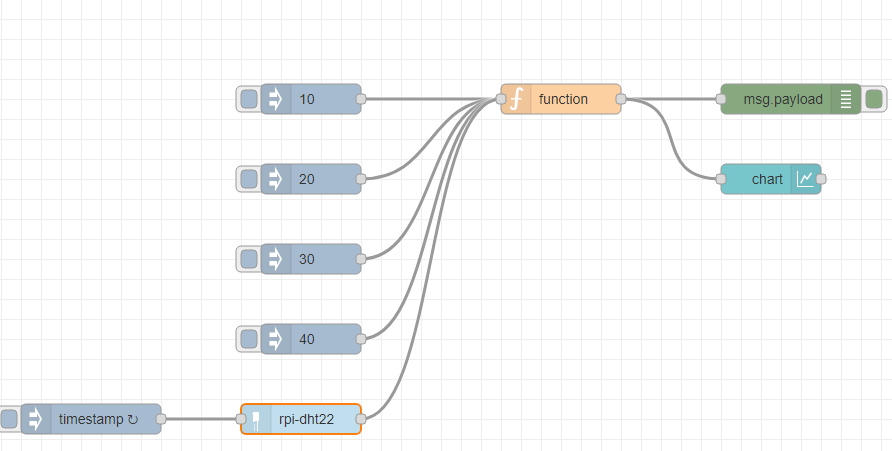
\includegraphics[width=0.35\textwidth]{fig/dht.png}
	\caption{A DHT szenzor programja.}
	\label{fig-dht}
\end{figure}

Sajnos a szenzor több beállítás után sem akart működni.

\chapter{Összefoglalás}

Összességében megismerkedtem a Raspberry PI-al, valamint a node-RED használatával. Ezek segítségével a jövőben szeretném 
továbbfejleszteni a projektmunkám/szakdolgozatom és egy könnyel elérhető kezelőfelületet létrehozni.

\end{document}
